\begin{figure}[t]
  \centering
  % Split the 720 bp-wide artwork at its midpoint to add space at the original scale.
  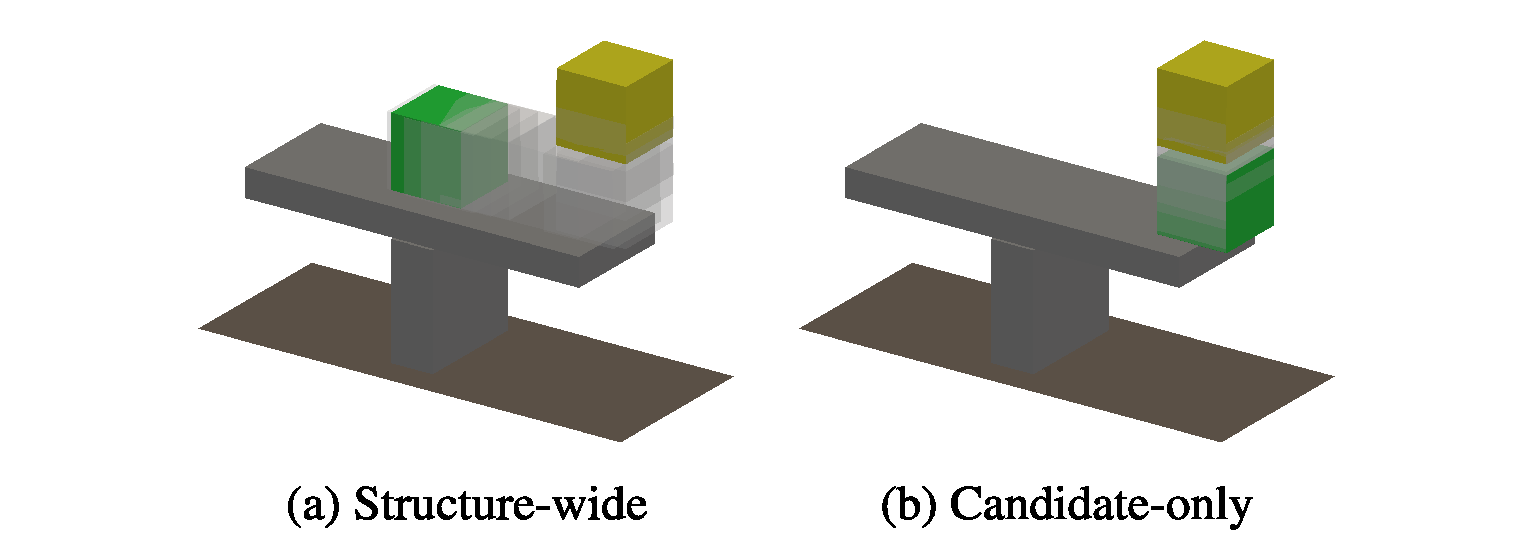
\includegraphics[width=0.475\columnwidth,trim=0 0 360bp 0,clip]{figures/pose_optimization_toy.eps}%
  \hspace{0.04\columnwidth}%
  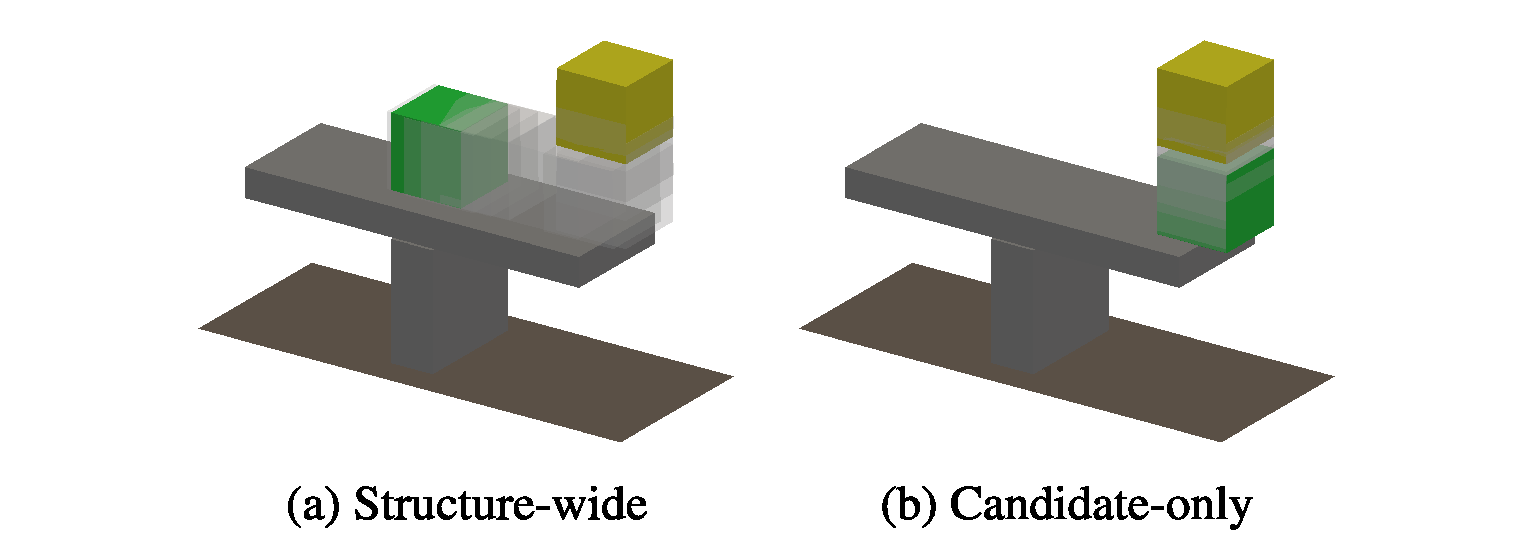
\includegraphics[width=0.475\columnwidth,trim=360bp 0 0 0,clip]{figures/pose_optimization_toy.eps}
  \caption{Seesaw example with initial (yellow), optimized (green), and intermediate (gray) poses. Evaluating equilibrium across the entire structure (a) moves the candidate toward the support. Candidate-only equilibrium (b) leaves it near the unsupported end.}
  \label{fig:pose_optimization_toy}
\end{figure}
